\section{Results}
The performance of our algorithm is demonstrated on \philbs \ and \rphumanserum.
Please refer to section S\ref{S-sec:algorithm_performance} for all other datasets.
For each comparison, the unregularized case is not smoothed, effectively $\lambda = 0$,
the partially regularized case uses the grid search fitted values of $\mathbf{\tau}$ but
uses a fixed $\lambda = 0.2$, and the fully regularized case uses the grid search fitted
values of both $\mathbf{\tau}$ and $\lambda$.

\subsection{Chromatogram Assignment Performance for \philbs}
    The fitted parameters for the network constructed for \philbs are shown in
    Table~\ref{tab:philbs_parameters}. The assigned chromatograms are shown in
    Figure~\ref{fig:philbs_assignments}. We observe up to seven branch structures in
    this sample, consistent with these \nglycans being derived from an avian context
    (\cite{Stanley2009,Khatri2016a}).

    \begin{table}[!htb]
        \small
        \centering
        \begin{threeparttable}
            \caption{Fitted $\lambda$, $\gamma$, and $\mathbf{\tau}$ for
                     \philbs \label{tab:philbs_parameters}}
            \begin{tabular}{l l}
                \toprule    
                Neighborhood Name & $\tau_i$ \\
                \midrule
                high-mannose & 17.615084 \\
                hybrid & 13.599120 \\
                bi-antennary & 0.0 \\
                asialo-bi-antennary & 13.919251 \\
                tri-antennary & 0.0 \\
                asialo-tri-antennary & 12.906467 \\
                tetra-antennary & 0.0 \\
                asialo-tetra-antennary & 14.723146 \\
                penta-antennary & 0.0 \\
                asialo-penta-antennary & 11.226188 \\
                hexa-antennary & 0.0 \\
                asialo-hexa-antennary & 10.696785 \\
                hepta-antennary & 0.0 \\
                asialo-hepta-antennary & 3.071313 \\
                \bottomrule
            \end{tabular}
            \begin{tablenotes}[normal]
                \item Fitted $\lambda = 0.99$ and $\gamma = 11.12$.
            \end{tablenotes}
        \end{threeparttable}
        \hspace{1em}
        \begin{threeparttable}
            \caption{Fitted $\lambda$, $\gamma$, and $\mathbf{\tau}$ for
                     \phil \label{tab:philbs_parameters}}
            \begin{tabular}{l l}
                \toprule    
                Neighborhood Name & $\tau_i$ \\
                \midrule
                high-mannose & 17.076439 \\
                hybrid & 13.706498 \\
                bi-antennary & 0.0 \\
                asialo-bi-antennary & 16.624051 \\
                tri-antennary &  0.0 \\
                asialo-tri-antennary & 15.671840 \\
                tetra-antennary & 0.0 \\
                asialo-tetra-antennary & 7.949766 \\
                penta-antennary & 0.0 \\
                asialo-penta-antennary & 0.0 \\
                hexa-antennary & 0.0 \\
                asialo-hexa-antennary & 0.0 \\
                hepta-antennary & 0.0 \\
                asialo-hepta-antennary & 0.0 \\
                \bottomrule
            \end{tabular}
            \begin{tablenotes}[normal]
                \item Fitted $\lambda = 0.99$ and $\gamma = 16.26$.
            \end{tablenotes}
        \end{threeparttable}
        \hspace{1em}
        \begin{threeparttable}
            \caption{Fitted $\lambda$, $\gamma$, and $\mathbf{\tau}$ for
                     \rpserum \label{tab:rpserum_parameters}}
            \begin{tabular}{l l}
                \toprule    
                Neighborhood Name & $\tau_i$ \\
                \midrule
                high-mannose & 19.839321 \\
                hybrid & 20.154402 \\
                bi-antennary & 19.288264 \\
                asialo-bi-antennary & 21.339077 \\
                tri-antennary & 22.502435 \\
                asialo-tri-antennary & 19.923334 \\
                tetra-antennary & 15.617820 \\
                asialo-tetra-antennary & 3.509291 \\
                penta-antennary & 8.764010 \\
                asialo-penta-antennary & 4.244343 \\
                hexa-antennary & 0.000000 \\
                asialo-hexa-antennary & 0.000000 \\
                hepta-antennary & 0.000000 \\
                asialo-hepta-antennary & 0.000000 \\
                \bottomrule
            \end{tabular}
            \begin{tablenotes}[normal]
                \item Fitted $\lambda = 0.99$ and $\gamma = 18.962$.
            \end{tablenotes}
        \end{threeparttable}
    \end{table}

    \begin{figure}[!htb]
        \caption{Chromatogram Assignments and Quantification
                 for \philbs\label{fig:philbs_assignments}}
        \centering
        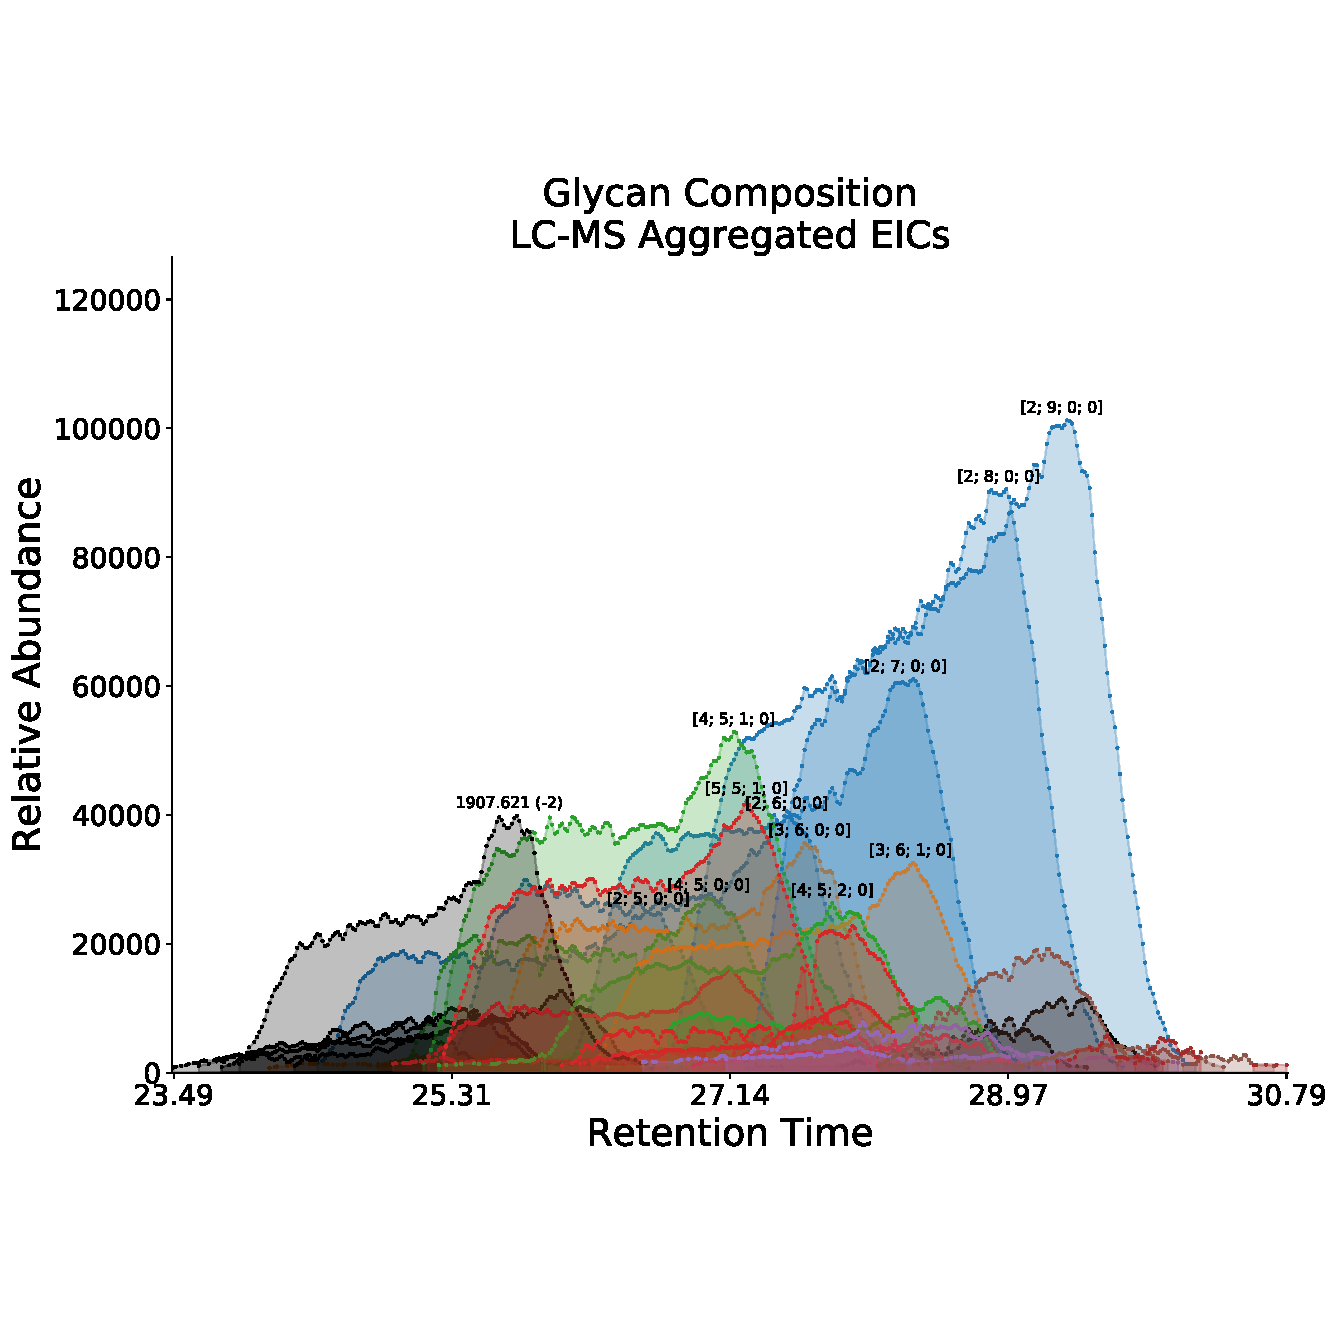
\includegraphics[width=0.45\textwidth,valign=t]{figure/phil_bs_chromatograms.pdf}
        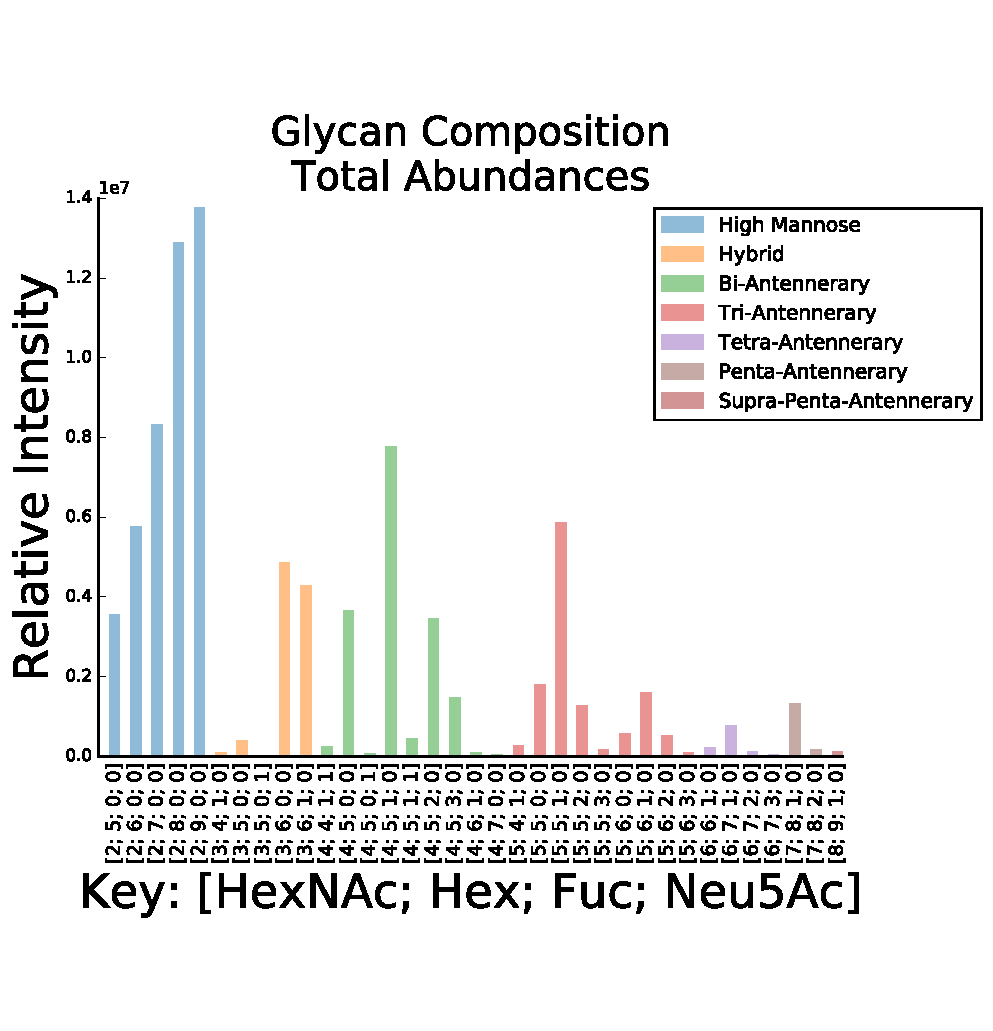
\includegraphics[width=0.45\textwidth,valign=t]{figure/phil_bs_abundances.pdf}
    \end{figure}

    \begin{figure}[!htb]
        \caption{Performance Comparison with and without Network Smoothing for \philbs
                 \label{fig:philbs_perf}}
        \centering
        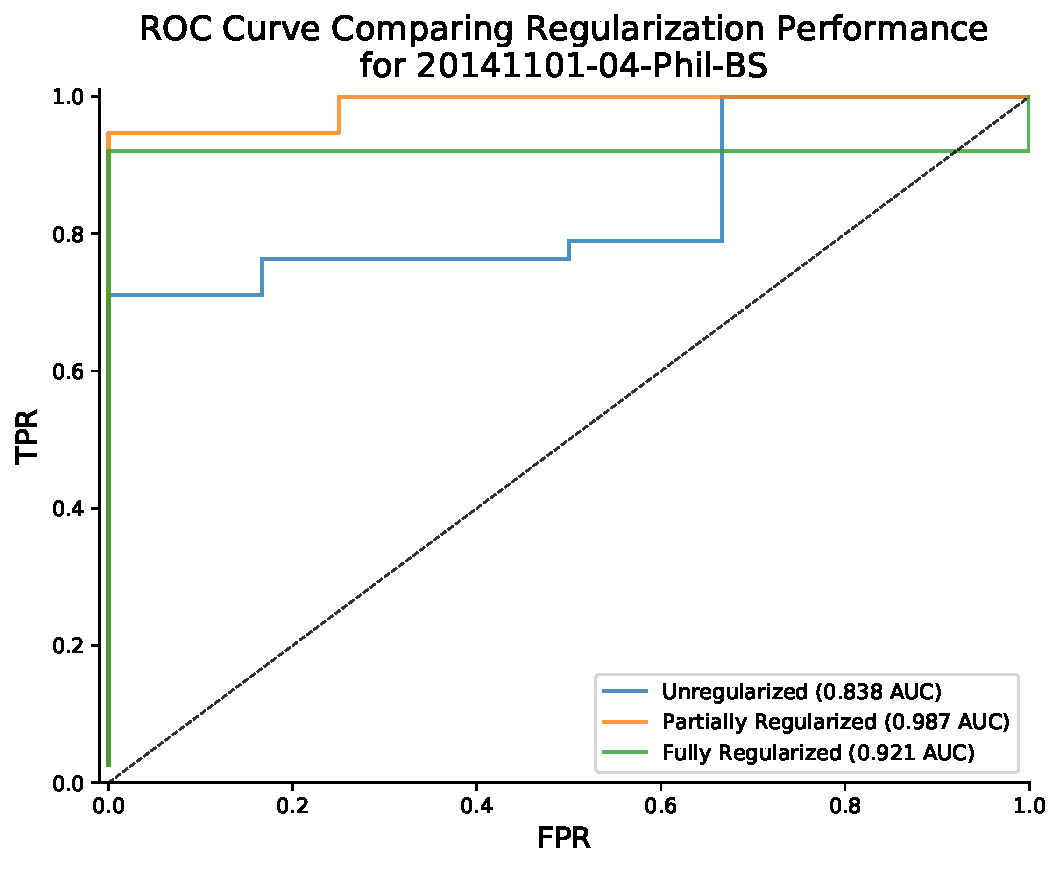
\includegraphics[width=0.42\textwidth,valign=t]{figure/phil_bs_native_roc.pdf}
        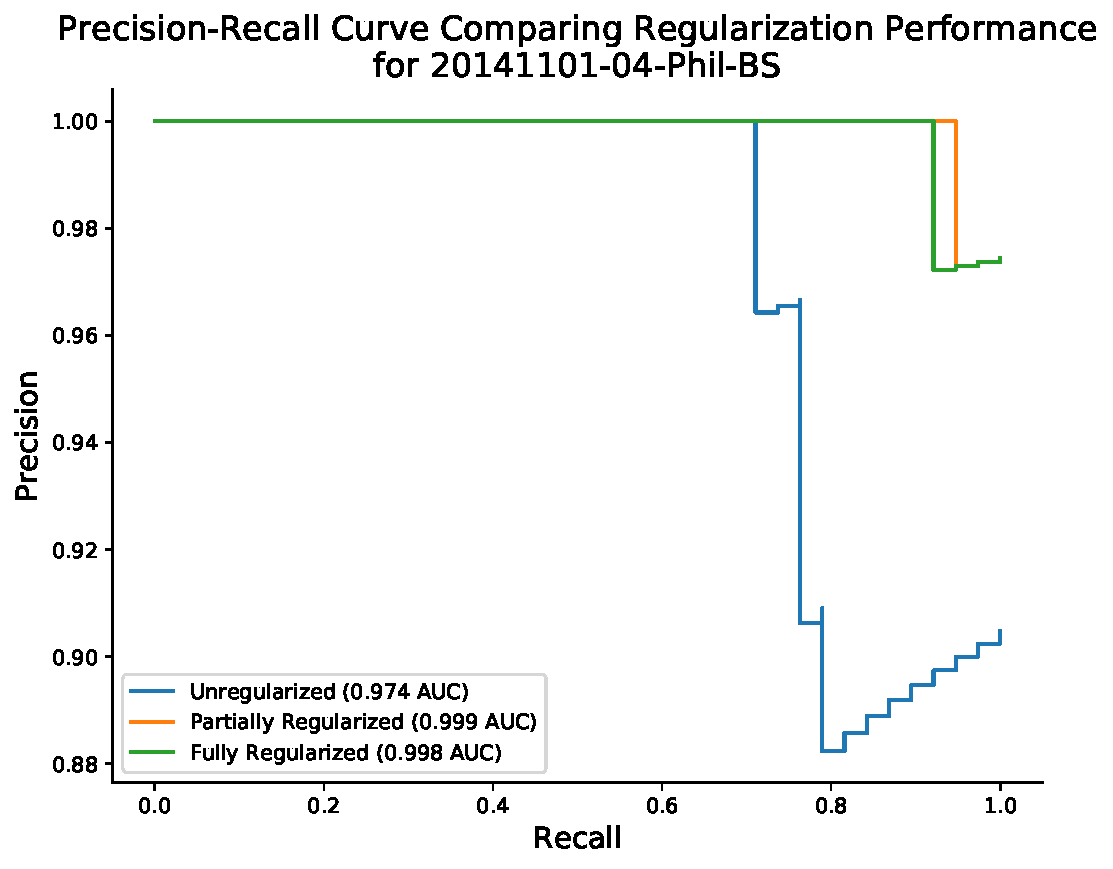
\includegraphics[width=0.45\textwidth,valign=t]{figure/phil_bs_native_prec_rec.pdf}
    \end{figure}

    The comparison of assignment performance with differing degrees of smoothing is
    shown in Figure~\ref{fig:philbs_perf}. The ROC AUC for the unregularized condition is
    0.838, for the partially regularized condition is 0.987, and for the fully regularized
    condition is 0.921. This demonstrates a higher true positive rate at the same false positive
    rate for both regularization conditions compared to the unregularized condition. In
    this condition, the Precision-Recall curve does not show a substantial difference in
    performance between conditions.

    \begin{table}[h]
        \centering
        \small
        \caption{Comparison of Performance on \philbs \ with Previous Analysis\label{tab:philbs_reanalysis_comparison}}
        \begin{threeparttable}
            \begin{tabular}{l l l l l}
                \toprule
                Method & \multicolumn{2}{l}{With Asialo-sulfated} & \multicolumn{2}{l}{Without Asialo-sulfated} \\
                \cmidrule(lr){2-3} \cmidrule(lr){4-5}
                & Reported & Validated & Reported & Validated \\
                \midrule
                Current Method \tnote{1} & 62 &   62  & 42 & 42 \\
                \cite{Khatri2016a} & 145 & 46 & 136 & 40\\
                \bottomrule
            \end{tabular}
            \begin{tablenotes}
                \item[1] Using partial regularization with $\lambda = 0.2$ and selected at $\phi_o > 5.0$
            \end{tablenotes}
        \end{threeparttable}
    \end{table}

\subsection{Chromatogram Assignment Performance for \rpserum}
    The fitted parameters for the network constructed for \rpserum \ are shown in
    Table~\ref{tab:rpserum_parameters}. The assigned chromatograms are shown in
    Figure~\ref{fig:rpserum_assignments}.

    \begin{figure}[!htb]
        \centering
        \caption{Chromatogram Assignments for \rpserum\label{fig:rpserum_assignments}}
        \begin{minipage}{0.45\linewidth}
            \centering
            \vspace{0pt}
            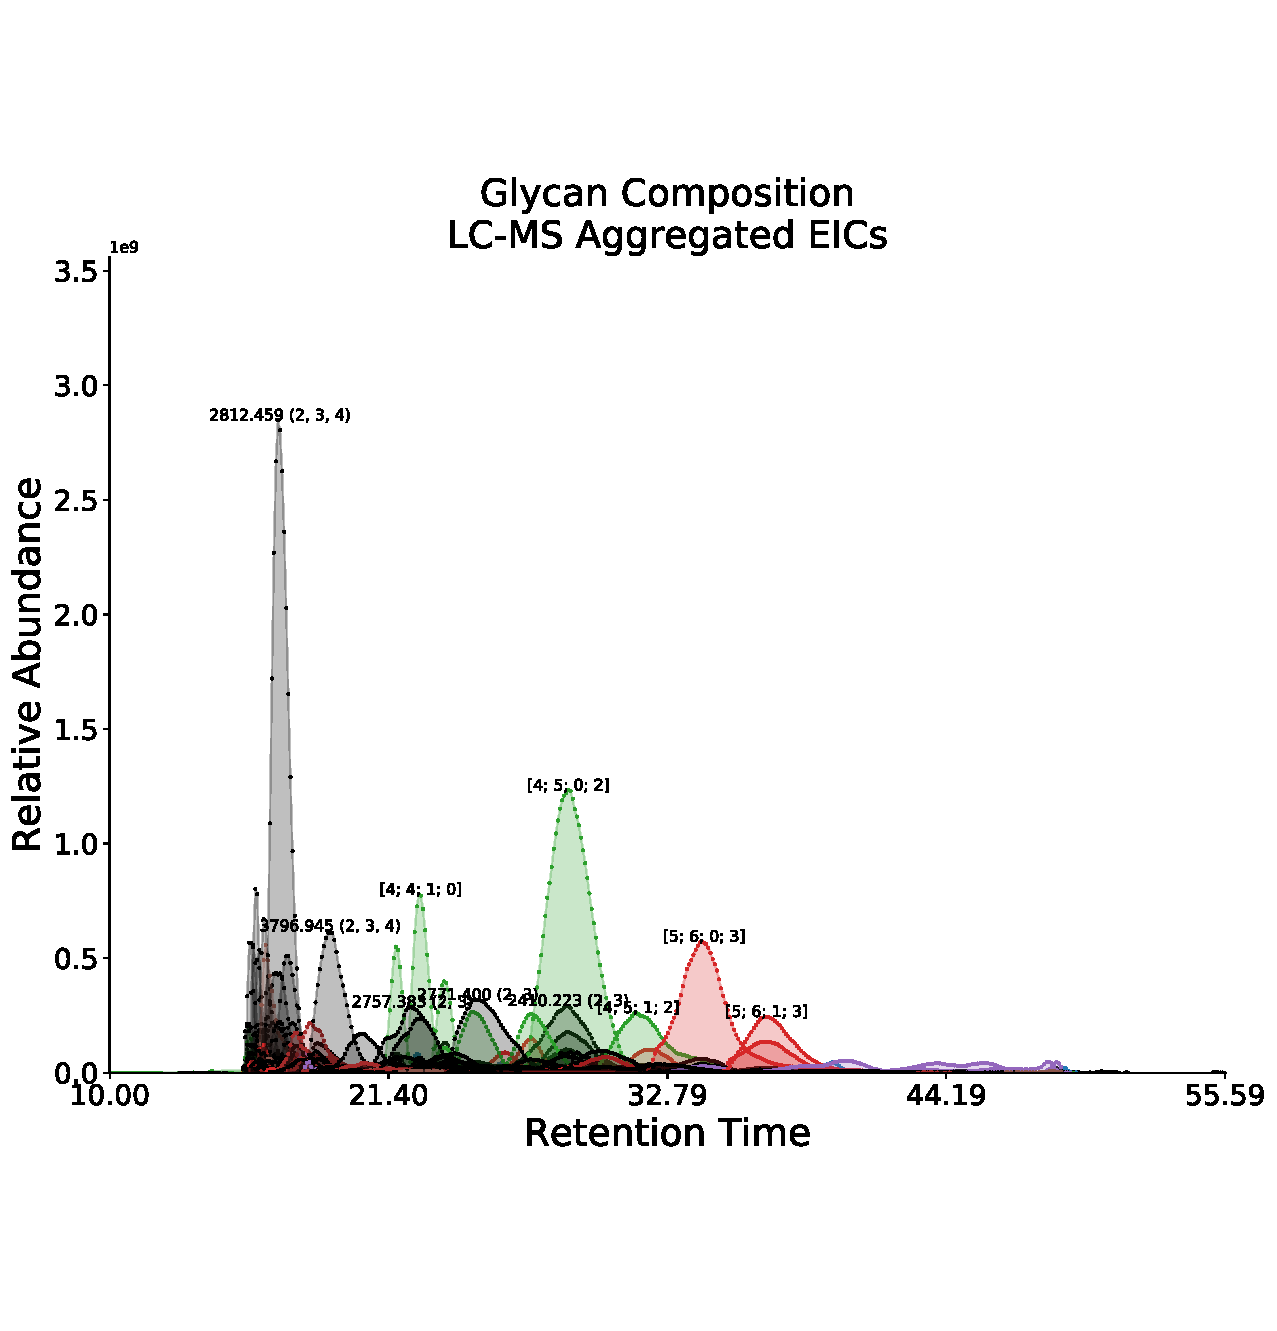
\includegraphics[width=\linewidth]{figure/rp_serum_chromatograms.pdf}
            \subcaption{Features Assigned After Grid Regularization of \rpserum\label{fig:rpserum_assignment:a}.
            Layout not finalized}
        \end{minipage}
        \begin{minipage}{0.45\linewidth}
            \centering
            \begin{subfigure}[t]{\linewidth}  
                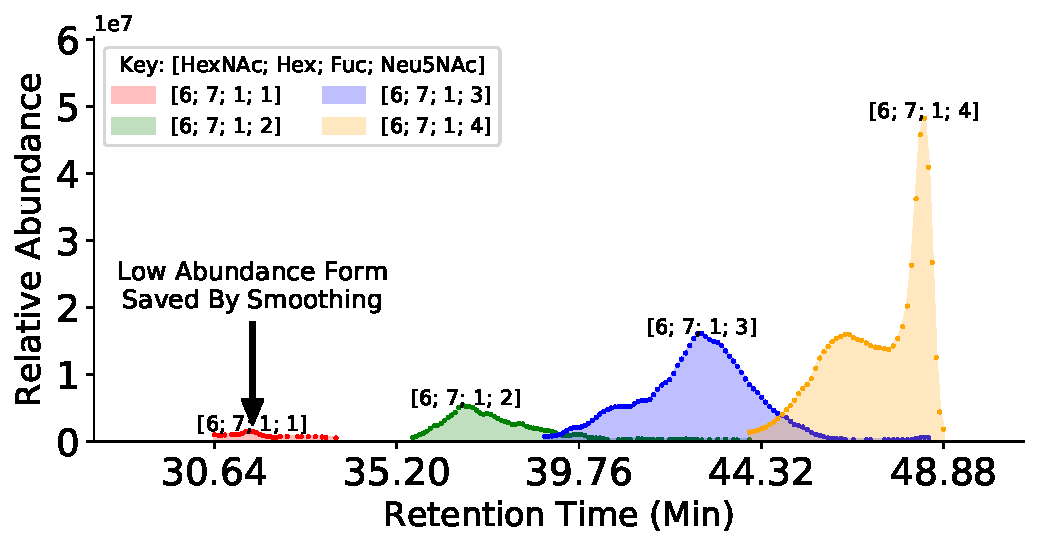
\includegraphics[width=0.75\linewidth, valign=t]{figure/fucosylated_tetra_antennary_structures.pdf}
                \subcaption{
                    Low scoring features which may be discarded based on individual evidence alone
                    may be more reasonable to accept given evidence from related composition, such
                    as our network smoothing method.\label{fig:rpserum_assignment:b}
                }
            \end{subfigure}

            \begin{subfigure}[t]{\linewidth}
                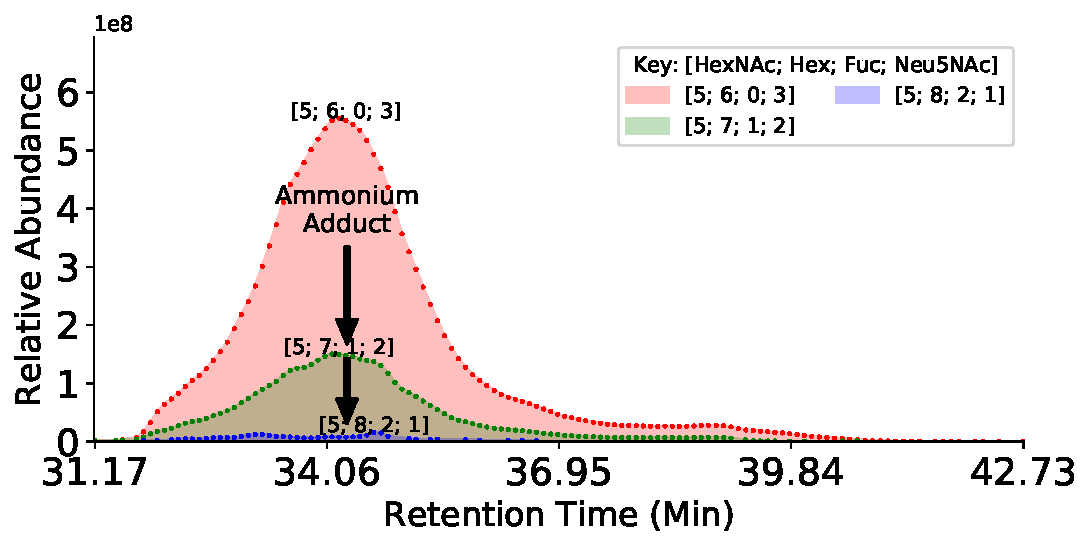
\includegraphics[width=0.75\linewidth, valign=t]{figure/ammonium_adduct_ambiguity.pdf}
                \subcaption{
                    This sample contains heavy ammonium adduction which introduces ambiguity
                    in intact mass based assignments.\label{fig:rpserum_assignment:c}
                }
            \end{subfigure}
        \end{minipage}
    \end{figure}

    \begin{figure}[htb]
        \caption{Performance Comparison with and without Network Smoothing for \rpserum
                 \label{fig:rpserum_perf}}
        \centering
        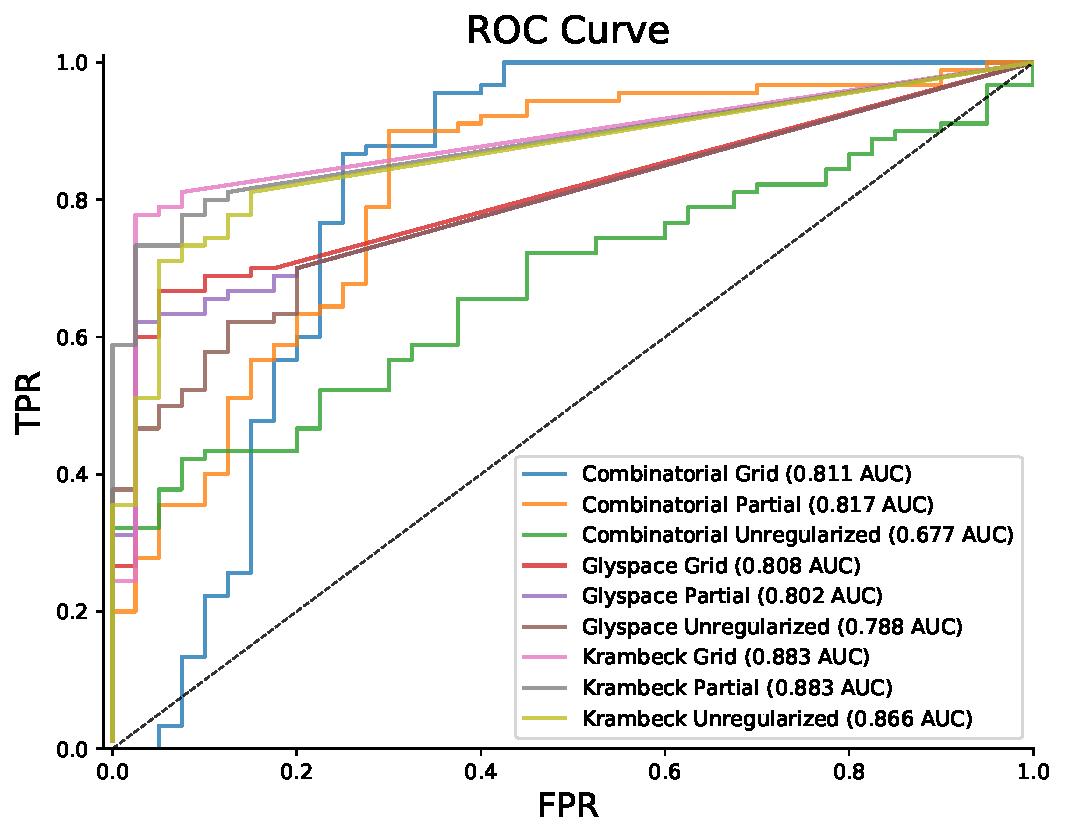
\includegraphics[width=0.42\textwidth,valign=t]{figure/serum_roc.pdf}
        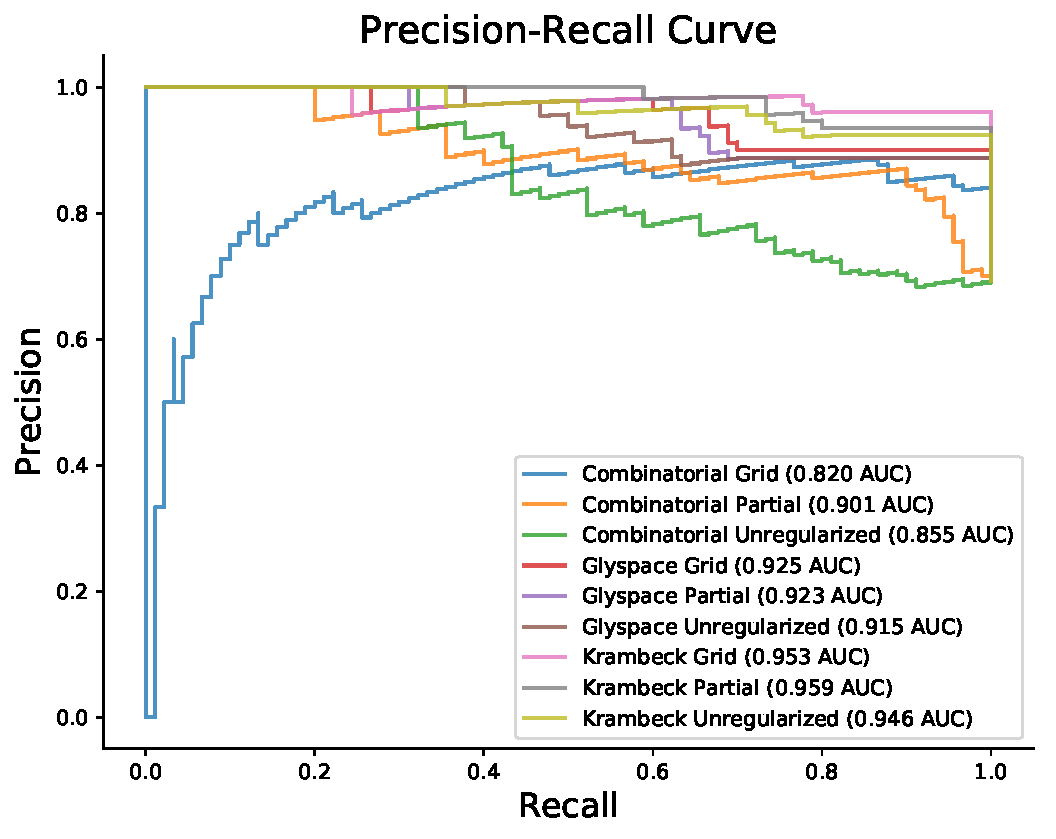
\includegraphics[width=0.45\textwidth,valign=t]{figure/serum_prec_rec.pdf}
    \end{figure}

    The comparison of assignment performance with differing degrees of smoothing is
    shown in Figure~\ref{fig:rpserum_perf}. The ROC AUC for the unregularized condition
    is 0.687, for the partially regularized condition is 0.831, and for the fully
    regularized condition is 0.797. The Precision-Recall AUC for the unregularized condition
    is 0.863, for the partially regularized condition is 0.913, and for the fully regularized
    condition is 0.838. This demonstrates that the partially regularized condition has superior
    performance to the unregularized and fully regularized conditions. This is complicated by
    the redundancies caused by ammonium adduction, but without high quality \msn \ this cannot
    be resolved.
